\usetikzlibrary{arrows}
\usetikzlibrary{positioning}

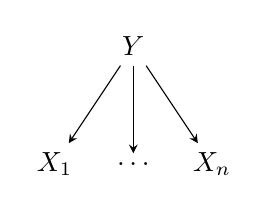
\begin{tikzpicture}[>=stealth]
    \node (Y) at (0,0) {$Y$};
    \node (X1) [below of=Y, node distance=1.5cm, xshift=-1cm] {$X_1$};
    \node (Xdots) [below of=Y, node distance=1.5cm, xshift=0cm] {$\dots$};
    \node (Xn) [below of=Y, node distance=1.5cm, xshift=1cm] {$X_n$};
    
    \draw[->] (Y) -- (X1);
    \draw[->] (Y) -- (Xdots);
    \draw[->] (Y) -- (Xn);
\end{tikzpicture}